%%%%%%%%%%%%%%%%%%%%%%%%%%%%%%%%%%%%%%%%%%%%%%%%%%%%%%
%% Modelo de Artigo do TCC - Técnico de Informática %%
%% Padrão ABNT IFF - Itaperuna (Artigo)             %%
%% Alterar apenas a parte indicada                  %%
%%%%%%%%%%%%%%%%%%%%%%%%%%%%%%%%%%%%%%%%%%%%%%%%%%%%%%
\documentclass[a4paper,12pt]{article}
% Definição da Linguagem (Não alterar!)
\usepackage[brazilian]{babel}

% Definição das margens (Não alterar!)
\usepackage[lmargin=3cm,tmargin=3cm,rmargin=2cm,bmargin=2cm]{geometry}

% Pacotes importantes (Não alterar!)
\usepackage{graphicx,xcolor,comment,enumerate,multirow,multicol,indentfirst}
\usepackage{amsmath,amsthm,amsfonts,amssymb,dsfont,mathtools,blindtext}
\usepackage{titlesec}
\usepackage[colorlinks=true, allcolors=blue]{hyperref}
\usepackage[font=footnotesize]{caption}
\usepackage{authblk}
\usepackage[onehalfspacing]{setspace}
\usepackage[natbibapa]{apacite}
\renewcommand\BBAA{e}
\renewcommand\BBAB{e}
\newenvironment{citacaolonga}
{\vspace{1cm}\hfill\begin{minipage}[c]{12cm}\setstretch{1}\small}
{\end{minipage}\vspace{1cm}}
\newenvironment{resumo}
{\begin{minipage}{\linewidth}\setstretch{1}}
{\end{minipage}\setstretch{1.5}}
\titlespacing{\section}{0pt}{1.5cm}{1.5cm}
\titlespacing{\subsection}{0pt}{1.5cm}{1.5cm}


\title{
    
\includegraphics[width=100px]{logo/logo.png}\\\large
    INSTITUTO FEDERAL DE EDUCAÇÃO, CIÊNCIA E TECNOLOGIA FLUMINENSE, CAMPUS ITAPERUNA\\\large
    %%%%%%%%%%%%%%%%%%%%%%%%%%%%%%%%%%%%%%%%%%%
    %% Coloque aqui o título do seu trabalho %%
    %%%%%%%%%%%%%%%%%%%%%%%%%%%%%%%%%%%%%%%%%%%
    MODELO DE TCC DO CURSO TÉCNICO DE INFORMÁTICA CAMPUS - ITAPERUNA
 }
%%%%%%%%%%%%%%%%%%%%%%%%%%%%%%%%%%
%% Colocar os nomes dos Autores %%
%%%%%%%%%%%%%%%%%%%%%%%%%%%%%%%%%%
\author{
Autor 1 \qquad 
Autor 2 \qquad
Autor 3 \qquad
Autor 4 \\
%%%%%%%%%%%%%%%%%%%%%%%%%%%%%%%%%%
%% Colocar o nome do orientador %%
%%%%%%%%%%%%%%%%%%%%%%%%%%%%%%%%%%
Orientador: Prof. Fulano de Tal
}
%%%%%%%%%%%%%%%%%%%%%%%%%%%%%%%%%%%%%%%%%%%
%% Colocar a data do projeto: mês e anos %%
%%%%%%%%%%%%%%%%%%%%%%%%%%%%%%%%%%%%%%%%%%%
\date{\small Itaperuna, 2023}

\begin{document}
\maketitle
\begin{abstract}
\begin{spacing}{1}
\noindent 
%%%%%%%%%%%%%%%%%%%%%%%%%%%%%%%%%
% Escreva o resumo do trabalho %%
%%%%%%%%%%%%%%%%%%%%%%%%%%%%%%%%%
O Trabalho de TCC é comumente elaborado no último ano do Curso Técnico do Instituto Federal Fluminense com objetivo de ensinar o aluno como elaborar um projeto acadêmico. As principais tarefas de qualquer TCC são: apoio a escolha do tema; encaminhamento aos orientadores; elaboração de um cronograma organizacional para execução das etapas; documentação formal acadêmica; e conclusão do projeto. Todas estas etapas em geral, são muito desgastantes pois a inexperiência dos alunos em produzir documentos formais podem desmotivar e até mesmo impedir a conclusão adequada de um projeto de conclusão de curso. Este documento tem o propósito de orientar os alunos do Curso Técnico de Informática na elaboração dos TCCs com maior qualidade e de forma padronizada, disponibilizando um modelo que facilitará a visualização com relação à apresentação gráfica. Para realizar esse apoio, este mesmo documento servirá como base para o Modelo \textit{LATEX}\footnote{LaTeX é um sistema ou programa de marcação para a editoração de documentos de alta qualidade tipográfica, específico para a elaboração de textos científicos. Trata-se de um conjunto de macros ou marcações para o processador de textos TeX}, o corpo textual poderá servir como exemplo de elaboração de um texto formal na ABNT \footnote{A Associação Brasileira de Normas Técnicas ou ABNT é uma entidade privada e sem fins lucrativos que cuida de diferentes normatizações no país. Ou seja, ela estuda e propõe formas de sistematizar processos, sejam eles de cunho acadêmico, tecnológico, industrial, produção de serviços, entre outros.} 
e a sintaxe utilizada para a sua criação, servirá de material de consulta tecnológica da ferramenta.

\noindent\textbf{Palavras-Chave:}
%%%%%%%%%%%%%%%%%%%%%%%%%%%%%%%%%%%%%%%%%%%%%%%%
%% Escreva as palavras chaves do seu trabalho %%
%%%%%%%%%%%%%%%%%%%%%%%%%%%%%%%%%%%%%%%%%%%%%%%%
TCC, ABNT, Latex
\end{spacing}
\end{abstract}
\newpage

%%%%%%%%%%%%%%%%%%%%%%%%%%%%%%%%%%%%%
% Escreva a introdução do trabalho %%
%%%%%%%%%%%%%%%%%%%%%%%%%%%%%%%%%%%%%
\section{Introdução}

A apresentação do documento escolhido como padrão dos TCCs neste curso Técnico de Informática é baseado em um modelo de artigo. Os motivos para esta escolha são: a redução do volume textual, a simplificação das regras técnicas para a criação dos documentos acadêmicos e ainda assim a manutenção das etapas necessárias para a criação de um projeto básico na área de tecnologia.

Uma definição simplificada de artigo pode ser entendida como:

%% Exemplo de citação longa %%
\begin{citacaolonga}
"Apresenta, de forma reduzida, uma pesquisa concluída. Os artigos são textos publicados em revistas científicas (periódicos científicos). É condição para publicação a efetiva relevância da pesquisa para a área específica. Além disso, devem apresentar a problemática pesquisada, os objetivos, a abordagem teórico-metodológica utilizada e a discussão dos resultados obtidos. No Brasil, os artigos são avaliados, de acordo com o mérito acadêmico pelo sistema Qualis Capes." \citep{petermann2020escrita}
\end{citacaolonga}

Assim como a citação longa acima, referencia bibliograficamente um trecho de um livro corretamente formatado dentro da ABNT e portanto poderá ser utilizado como exemplo para a construção de outros trabalhos, diversos outros exemplos serão apresentados ao longo das seções demonstrando como inserir figuras, tabelas e etc.

Segundo \citet{botelho2021praticas}, introdução deve ser a primeira seção numerada do seu trabalho, ela precisa demonstrar uma visão geral do seu projeto ainda sem os métodos e detalhes de desenvolvimento. Apenas poucos parágrafos são suficientes. Aproveite para descrever rapidamente a importância do seu trabalho, qual a relevância em pesquisar e desenvolver seu software.

Nesta seção você deve descrever uma breve visão histórica da área de seu estudo, a especificação de seu projeto dentro do escopo tecnológico abordado com uma revisão da literatura. Aproveite este momento para descrever os seus objetivos pretendidos.
%Fim da Introdução

%%%%%%%%%%%%%%%%%%%%%%%%%%%%%%%%%%%%%%%%%%%%%%%%%%%%%%
%% O Trabalho deve ter uma seção de desenvolvimento %%
%%%%%%%%%%%%%%%%%%%%%%%%%%%%%%%%%%%%%%%%%%%%%%%%%%%%%%
\section{Desenvolvimento}

O primeiro ponto a ser abordado no corpo do artigo é a definição do problema \cite{zeroum}. Explique os conceitos básicos, os termos usados e estabeleça claramente os objetivos e as hipóteses. O próximo passo é informar sobre materiais e métodos. Os procedimentos metodológicos empregados para o levantamento de dados e sua análise devem estar claramente apresentados. Aproveite este momento para estabelecer suas pesquisas e os caminhos escolhidos para abordagem dos problemas.

A seguir, apresenta-se a discussão: utilize argumentos convincentes e adequados, prova matemática, exemplos, equações, análises estatísticas, padrões/tendências observadas, opiniões e ideias, além da coleção de números coletados e tabelados. No caso específico da Informática, aproveite para apresentar as ferramentas de desenvolvimento e se julgar necessário, apresente trechos relevantes dos códigos desenvolvidos.

Também é necessário realizar comparações com resultados, assim como Sugerir aplicações para o seu trabalho. Retome os objetivos de seu trabalho e discuta a significância dos resultados obtidos.
Gráficos e tabelas devem sempre ter fonte e legendas (letra tamanho 10pt), dizendo exatamente o que representam, aparecendo sempre junto ao texto a que se
referem.

%%%%%%%%%%%%%%%%%%%%%%%%%%%%%%%%%%%%%%%%%%%%%%%%%%%%%%%%%%%%%%%%%%%%%%%%
%% Estas subseções não devem ser incluídas no trabalho final          %%
%% Apenas estão aqui para orientar como utilizar a ferramenta LATEX.  %%
%%%%%%%%%%%%%%%%%%%%%%%%%%%%%%%%%%%%%%%%%%%%%%%%%%%%%%%%%%%%%%%%%%%%%%%%
\subsection{A escolha de um tema e seu orientador}

Em geral, a tarefa mais difícil de um trabalho é definir um tema de projeto. Isto acontece pois duas coisas são fundamentais para o desenvolvimento deste tema: o \textbf{interesse} do aluno e a \textbf{disponibilidade} de um orientador.

No intuito de ajudar os alunos, é recomendado que os mesmos procurem os professores orientadores previamente para tomarem conhecimento de suas áreas de estudo antes de proporem novos temas. Assim poderão ter maior clareza sobre os possíveis projetos que poderão participar de acordo com os interesses mútuos.

Caso não exista um consenso, pode ser necessário a busca do coordenador do curso ou do professor da disciplina de \underline{Práticas Profissionais II}, que poderão auxiliar no entendimento do grupo adequando as ideias e determinando o orientador disponível à atender o aluno.

Como é observado, a escolha do tema e do orientador é uma tarefa de entendimento social entre o interesse do grupo e do orientador, mas em última análise, cabe sempre ao orientador dar a palavra final, uma vez que ele é o detentor do conhecimento específico da área a ser estudada.

Para exemplificar, podemos observar este trecho do Manual de TCC para Graduação de Engenharia do campus de Macaé: "De preferência deverá ser um professor que tem um conhecimento aprofundado no tema em foco e se vê comprometido com a questão. A ele cabe assessorar seu orientando em todas as etapas da construção do trabalho." \citep{botelho2021praticas}.


%%%%%%%%%%%%%%%%%%%%%%%%%%%%%%%%%%%%%%%%%%%%%%%%%%%%%%%%%%%%%%%%%%%%%%%%
%% Estas subseções não devem ser incluídas no trabalho final          %%
%% Apenas estão aqui para orientar como utilizar a ferramenta LATEX.  %%
%%%%%%%%%%%%%%%%%%%%%%%%%%%%%%%%%%%%%%%%%%%%%%%%%%%%%%%%%%%%%%%%%%%%%%%%
\subsection{Como incluir Figuras}

Primeiro, você precisa fazer upload do arquivo de imagem do seu computador usando o link de upload no menu de árvore de arquivos. Em seguida, use o comando includegraphics para incluí-lo em seu documento. Use o ambiente figure e o comando caption para adicionar um número e uma legenda à sua figura. Veja o código para a Figura.\ref{fig:frog} nesta seção como exemplo.

\begin{figure}[h]
\centering
\caption{Sapo Verde}
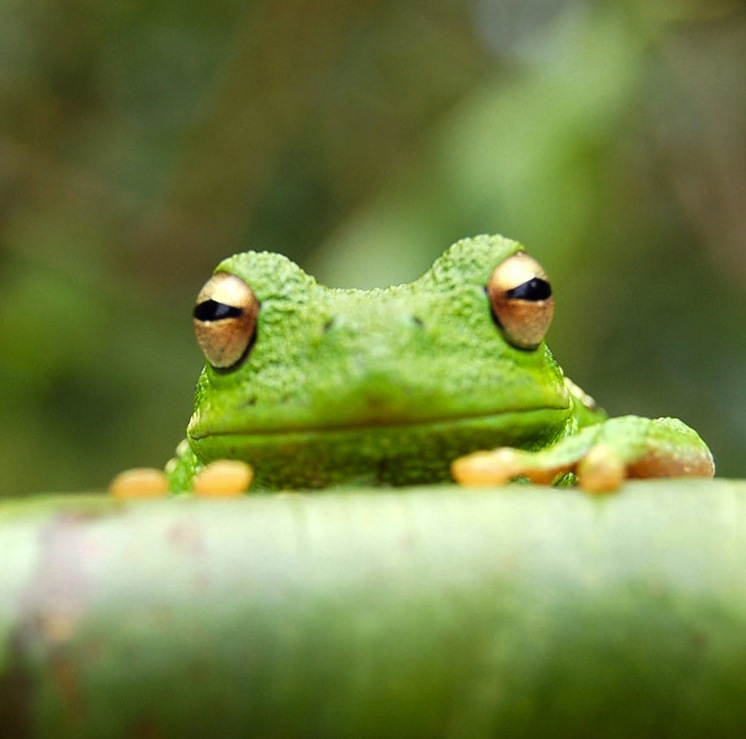
\includegraphics[width=0.3\textwidth]{frog.jpg}
\\\footnotesize{Uma imagem genérica de um sapo.}
\label{fig:frog}
\end{figure}

%%%%%%%%%%%%%%%%%%%%%%%%%%%%%%%%%%%%%%%%%%%%%%%%%%%%%%%%%%%%%%%%%%%%%%%%
%% Estas subseções não devem ser incluídas no trabalho final          %%
%% Apenas estão aqui para orientar como utilizar a ferramenta LATEX.  %%
%%%%%%%%%%%%%%%%%%%%%%%%%%%%%%%%%%%%%%%%%%%%%%%%%%%%%%%%%%%%%%%%%%%%%%%%
\subsection{Como adicionar Tabelas}

Use os ambientes \textit{table} e \textit{tabular} para criar tabelas básicas - veja a Tabela \ref{tab:widgets}, como exemplo. Para mais informações, veja o \textit{help} no artigo: \href{https://www.overleaf.com/learn/latex/tables}{tables}. 

\begin{table}[h]
\centering
\caption{Tabela de Exemplo}
\begin{tabular}{|l|r|}
\hline
Descrição & Quantidade \\\hline
Caneta & 42 \\
Lápis & 13\\\hline
\end{tabular}
\\\footnotesize{Uma tabela genérica}
\label{tab:widgets}
\end{table}

%%%%%%%%%%%%%%%%%%%%%%%%%%%%%%%%%%%%%%%%%%%%%%%%%%%%%%%%%%%%%%%%%%%%%%%%
%% Estas subseções não devem ser incluídas no trabalho final          %%
%% Apenas estão aqui para orientar como utilizar a ferramenta LATEX.  %%
%%%%%%%%%%%%%%%%%%%%%%%%%%%%%%%%%%%%%%%%%%%%%%%%%%%%%%%%%%%%%%%%%%%%%%%%
\subsection{Como adicionar listas}

Vocês podem adicionar listas enumeradas \dots

\begin{enumerate}
\item Exemplo 1,
\item Exemplo 2.
\end{enumerate}
\dots ou pontos \dots
\begin{itemize}
\item Exemplo 3,
\item Exemplo 4.
\end{itemize}

%%%%%%%%%%%%%%%%%%%%%%%%%%%%%%%%%%%%%%%%%%%%%%%%%%%%%%%%%%%%%%%%%%%%%%%%
%% Estas subseções não devem ser incluídas no trabalho final          %%
%% Apenas estão aqui para orientar como utilizar a ferramenta LATEX.  %%
%%%%%%%%%%%%%%%%%%%%%%%%%%%%%%%%%%%%%%%%%%%%%%%%%%%%%%%%%%%%%%%%%%%%%%%%
\subsection{Como adicionar fórmulas}

\LaTeX{} é ótimo para compor fórmulas: $X_1, X_2, \ldots, X_n$ seja escrita ao longo do texto: $\text{E}[X_i] = \mu$ e $\text{Var}[X_i] = \sigma^2 < \infty$, ou enumeradas para referenciar:
\begin{equation}
  S_n = \frac{X_1 + X_2 + \cdots + X_n}{n}
      = \frac{1}{n}\sum_{i}^{n} X_i
\end{equation}

A seguir, podemos observar mais alguns exemplos de criação de fórmulas: $\sqrt{n}(S_n - \mu)$ e $\mathcal{N}(0, \sigma^2)$.

%%%%%%%%%%%%%%%%%%%%%%%%%%%%%%%%%%%%%%%%%%%%%%
%% Todo o trabalho precisa de uma conclusão %%
%%%%%%%%%%%%%%%%%%%%%%%%%%%%%%%%%%%%%%%%%%%%%%
\section{Conclusão}
A última seção enumerada de seu artigo é a conclusão. Ela deve ser construída  com os resultados apresentados ao longo do desenvolvimento do projeto. É fundamental que a conclusão seja objetiva para a clareza do alcance dos objetivos iniciais. Geralmente a conclusão trazem novas informações ao trabalho, elucidando tanto resultados afirmativos às hipóteses iniciais, quanto negações. Em ambos os casos, o trabalho terá valor, desde que a metodologia utilizada no desenvolvimento tenha sido adequada à abordagem do problema.
Deve-se assegurar que não tenham sido citadas conclusões que não foram objetivo do trabalho. É sempre muito importante que a conclusão apresente novas ideias para futuros trabalhos.

%% Não alterar nada %%
\bibliographystyle{apacite}
\bibliography{sample}

\end{document}